\documentclass[11pt]{article}
\usepackage[margin=2.5cm]{geometry}
\usepackage{amsmath,amssymb}
\usepackage{tikz}
\usetikzlibrary{arrows.meta,positioning,shapes,fit,calc,decorations.pathreplacing,backgrounds}
\usepackage{listings}
\usepackage{xcolor}
\usepackage{hyperref}
\usepackage{booktabs}

% Colors
\definecolor{dynamic}{RGB}{66,133,244}    % blue - dynamic/traced
\definecolor{static}{RGB}{234,67,53}      % red - static/baked
\definecolor{batch0}{RGB}{52,168,83}      % green - batch 0
\definecolor{batch1}{RGB}{66,133,244}     % blue - batch 1
\definecolor{batch2}{RGB}{234,67,53}      % red - batch 2
\definecolor{market}{RGB}{255,152,0}      % orange
\definecolor{network}{RGB}{156,39,176}    % purple
\definecolor{democracy}{RGB}{0,150,136}   % teal
\definecolor{codebg}{RGB}{245,245,245}

\lstset{
  language=Python,
  basicstyle=\small\ttfamily,
  keywordstyle=\color{blue},
  stringstyle=\color{red!70!black},
  commentstyle=\color{green!50!black},
  backgroundcolor=\color{codebg},
  frame=single,
  breaklines=true,
  columns=flexible,
}

\title{CI-Lib Core Primitives:\\Implementation Changelog}
\author{Jonas Hallgren\\Equilibria Network}
\date{March 2026}

\begin{document}
\maketitle

\begin{abstract}
This document records the implementation of CI-Lib's four core primitives:
\textsc{GraphState} (immutable typed state), \textsc{Transform} (pure functions with read/write declarations),
\textsc{Schedule} (temporal orchestration), and \textsc{Composition Operators}
(sequential, parallel, conditional). Each section includes architecture diagrams
and code excerpts.
\end{abstract}

\tableofcontents
\newpage

%% ================================================================
\section{GraphState Pytree Fix}

The foundational change: partitioning \texttt{global\_attrs} so JAX arrays
are traced (dynamic) and Python scalars are baked into the compiled kernel (static).

\subsection{Before and After}

\begin{center}
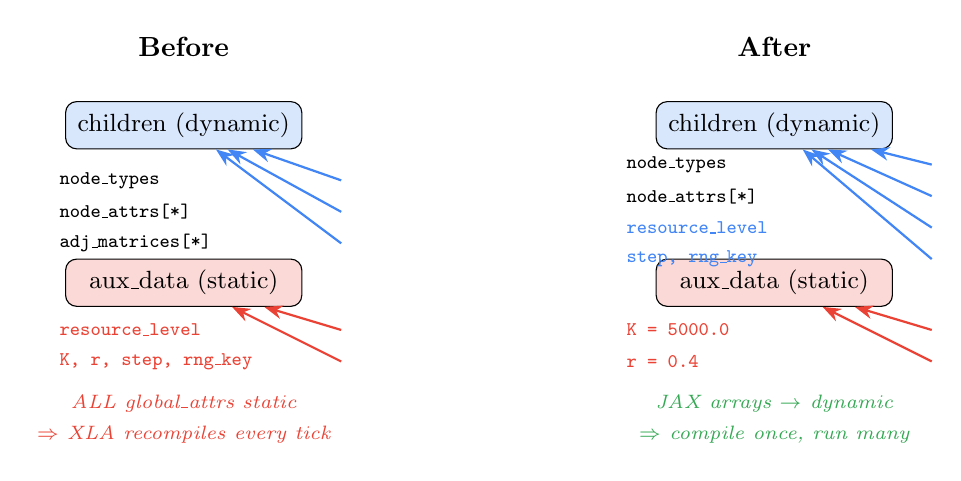
\begin{tikzpicture}[
  box/.style={draw, rounded corners, minimum width=3cm, minimum height=0.6cm, font=\small},
  arr/.style={-{Stealth}, thick},
]
% BEFORE
\node[font=\bfseries] at (-3.5, 3.5) {Before};
\node[box, fill=dynamic!20] (ch1) at (-3.5, 2.5) {children (dynamic)};
\node[box, fill=static!20] (aux1) at (-3.5, 0.5) {aux\_data (static)};

\node[font=\ttfamily\scriptsize, anchor=west] at (-5.2, 1.8) {node\_types};
\node[font=\ttfamily\scriptsize, anchor=west] at (-5.2, 1.4) {node\_attrs[*]};
\node[font=\ttfamily\scriptsize, anchor=west] at (-5.2, 1.0) {adj\_matrices[*]};

\draw[arr, dynamic] (-1.5, 1.8) -- (ch1);
\draw[arr, dynamic] (-1.5, 1.4) -- (ch1);
\draw[arr, dynamic] (-1.5, 1.0) -- (ch1);

\node[font=\ttfamily\scriptsize, anchor=west, text=static] at (-5.2, -0.1) {resource\_level};
\node[font=\ttfamily\scriptsize, anchor=west, text=static] at (-5.2, -0.5) {K, r, step, rng\_key};
\draw[arr, static] (-1.5, -0.1) -- (aux1);
\draw[arr, static] (-1.5, -0.5) -- (aux1);
\node[font=\scriptsize\itshape, text=static, anchor=north] at (-3.5, -0.8) {ALL global\_attrs static};
\node[font=\scriptsize\itshape, text=static, anchor=north] at (-3.5, -1.2) {$\Rightarrow$ XLA recompiles every tick};

% AFTER
\node[font=\bfseries] at (4, 3.5) {After};
\node[box, fill=dynamic!20] (ch2) at (4, 2.5) {children (dynamic)};
\node[box, fill=static!20] (aux2) at (4, 0.5) {aux\_data (static)};

\node[font=\ttfamily\scriptsize, anchor=west] at (2.0, 2.0) {node\_types};
\node[font=\ttfamily\scriptsize, anchor=west] at (2.0, 1.6) {node\_attrs[*]};
\node[font=\ttfamily\scriptsize, anchor=west, text=dynamic] at (2.0, 1.2) {resource\_level};
\node[font=\ttfamily\scriptsize, anchor=west, text=dynamic] at (2.0, 0.8) {step, rng\_key};

\node[font=\ttfamily\scriptsize, anchor=west, text=static] at (2.0, -0.1) {K = 5000.0};
\node[font=\ttfamily\scriptsize, anchor=west, text=static] at (2.0, -0.5) {r = 0.4};

\draw[arr, dynamic] (6.0, 2.0) -- (ch2);
\draw[arr, dynamic] (6.0, 1.6) -- (ch2);
\draw[arr, dynamic] (6.0, 1.2) -- (ch2);
\draw[arr, dynamic] (6.0, 0.8) -- (ch2);
\draw[arr, static] (6.0, -0.1) -- (aux2);
\draw[arr, static] (6.0, -0.5) -- (aux2);

\node[font=\scriptsize\itshape, text=batch0, anchor=north] at (4, -0.8) {JAX arrays $\to$ dynamic};
\node[font=\scriptsize\itshape, text=batch0, anchor=north] at (4, -1.2) {$\Rightarrow$ compile once, run many};
\end{tikzpicture}
\end{center}

\noindent\textbf{Partitioning rule:} \texttt{isinstance(v, (jnp.ndarray, jax.Array))} $\to$ children;
everything else $\to$ aux\_data. Impact: $\sim$3--10$\times$ speedup by eliminating per-tick recompilation.

%% ================================================================
\section{Typed Transforms}

The \texttt{@transform} decorator attaches read/write metadata to pure functions.

\begin{center}
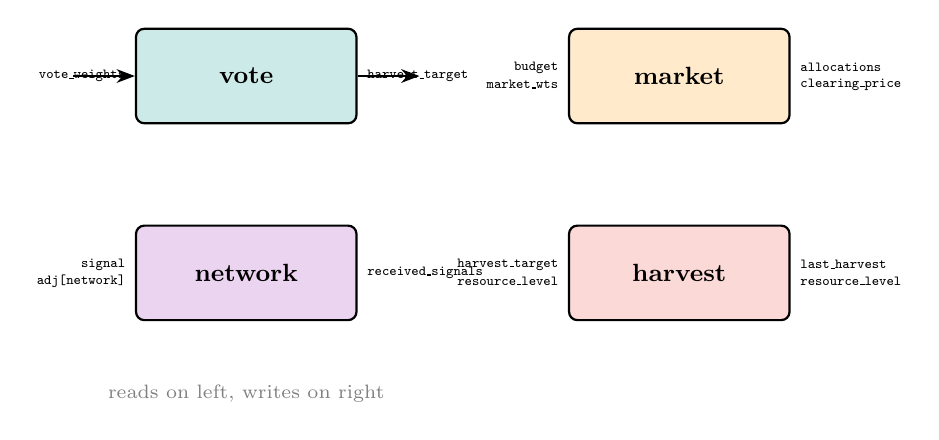
\begin{tikzpicture}[
  tbox/.style={draw, thick, rounded corners=3pt, minimum width=2.8cm, minimum height=1.2cm,
               font=\small\bfseries, align=center},
  port/.style={font=\tiny\ttfamily, anchor=east},
  portw/.style={font=\tiny\ttfamily, anchor=west},
]
% Vote
\node[tbox, fill=democracy!20] (vote) at (0,0) {vote};
\node[port] at (vote.west) {vote\_weights};
\node[portw] at (vote.east) {harvest\_target};
\draw[-{Stealth}, thick] (-2.2, 0) -- (vote.west);
\draw[-{Stealth}, thick] (vote.east) -- (2.2, 0);

% Market
\node[tbox, fill=market!20] (mkt) at (5.5,0) {market};
\node[port] at ([yshift=3pt]mkt.west) {budget};
\node[port] at ([yshift=-3pt]mkt.west) {market\_wts};
\node[portw] at ([yshift=3pt]mkt.east) {allocations};
\node[portw] at ([yshift=-3pt]mkt.east) {clearing\_price};

% Network
\node[tbox, fill=network!20] (net) at (0,-2.5) {network};
\node[port] at ([yshift=3pt]net.west) {signal};
\node[port] at ([yshift=-3pt]net.west) {adj[network]};
\node[portw] at (net.east) {received\_signals};

% Harvest
\node[tbox, fill=batch2!20] (harv) at (5.5,-2.5) {harvest};
\node[port] at ([yshift=3pt]harv.west) {harvest\_target};
\node[port] at ([yshift=-3pt]harv.west) {resource\_level};
\node[portw] at ([yshift=3pt]harv.east) {last\_harvest};
\node[portw] at ([yshift=-3pt]harv.east) {resource\_level};

% Labels
\node[font=\scriptsize, text=gray, anchor=north] at (0, -3.8) {reads on left, writes on right};
\end{tikzpicture}
\end{center}

\begin{lstlisting}
@transform(reads=["vote_weights"], writes=["harvest_target"])
def direct_democracy(state: GraphState) -> GraphState:
    ...
\end{lstlisting}

%% ================================================================
\section{Pipeline Compiler}

The compiler builds a dependency DAG from read/write sets, topologically sorts into
parallel batches, and composes into a single \textsc{Transform}.

\subsection{Dependency DAG}

\begin{center}
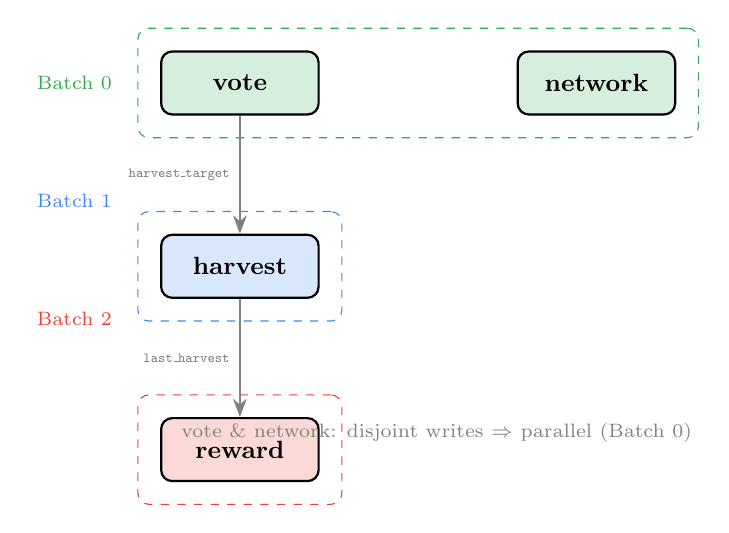
\begin{tikzpicture}[
  node distance=2cm,
  tnode/.style={draw, thick, rounded corners, minimum width=2cm, minimum height=0.8cm,
                font=\small\bfseries, align=center},
  dep/.style={-{Stealth}, thick, gray},
]
% Nodes
\node[tnode, fill=batch0!20] (vote) {vote};
\node[tnode, fill=batch0!20, right=2.5cm of vote] (net) {network};
\node[tnode, fill=batch1!20, below=1.5cm of vote] (harv) {harvest};
\node[tnode, fill=batch2!20, below=1.5cm of harv] (rew) {reward};

% Dependencies
\draw[dep] (vote) -- node[left, font=\tiny\ttfamily] {harvest\_target} (harv);
\draw[dep] (harv) -- node[left, font=\tiny\ttfamily] {last\_harvest} (rew);

% Batch labels
\node[font=\scriptsize, text=batch0, anchor=east] at (-1.5, 0) {Batch 0};
\node[font=\scriptsize, text=batch1, anchor=east] at (-1.5, -1.5) {Batch 1};
\node[font=\scriptsize, text=batch2, anchor=east] at (-1.5, -3.0) {Batch 2};

% Dashed batch boxes
\begin{scope}[on background layer]
  \node[draw=batch0, dashed, rounded corners, fit=(vote)(net), inner sep=8pt] {};
  \node[draw=batch1, dashed, rounded corners, fit=(harv), inner sep=8pt] {};
  \node[draw=batch2, dashed, rounded corners, fit=(rew), inner sep=8pt] {};
\end{scope}

% Note
\node[font=\scriptsize, text=gray, anchor=north] at (2.5, -4.2)
  {vote \& network: disjoint writes $\Rightarrow$ parallel (Batch 0)};
\end{tikzpicture}
\end{center}

\noindent\textbf{Algorithm:} Kahn's topological sort. At each step, collect \emph{all}
zero-in-degree nodes into one batch. Transforms within a batch run via \texttt{parallel()};
batches execute via \texttt{sequential()}.

\begin{lstlisting}
pipeline = compile_pipeline([vote, harvest, reward, network])
# Derived order: [vote || network] -> harvest -> reward
\end{lstlisting}

%% ================================================================
\section{Schedule Primitive}

The schedule maps clock ticks to active transforms. Each transform has a
\emph{cadence} $c_i$ and \emph{phase offset} $\phi_i$: it fires at tick $t$
iff $(t - \phi_i) \bmod c_i = 0$.

\subsection{Timeline Diagram}

\begin{center}
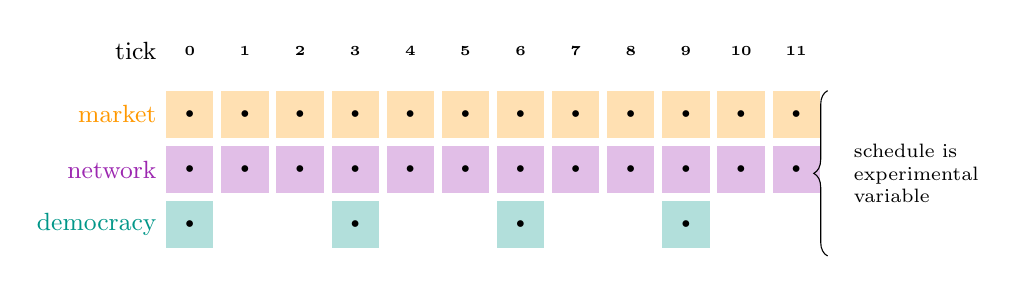
\begin{tikzpicture}[
  cell/.style={minimum width=0.6cm, minimum height=0.6cm, font=\tiny},
  active/.style={cell, fill=#1!30},
  inactive/.style={cell},
]
% Header
\foreach \t in {0,...,11} {
  \node[cell, font=\tiny\bfseries] at (\t*0.7, 0.8) {\t};
}
\node[font=\small, anchor=east] at (-0.3, 0.8) {tick};

% Market (cadence=1)
\node[font=\small, anchor=east, text=market] at (-0.3, 0) {market};
\foreach \t in {0,...,11} {
  \node[active=market] at (\t*0.7, 0) {$\bullet$};
}

% Network (cadence=1)
\node[font=\small, anchor=east, text=network] at (-0.3, -0.7) {network};
\foreach \t in {0,...,11} {
  \node[active=network] at (\t*0.7, -0.7) {$\bullet$};
}

% Democracy (cadence=3)
\node[font=\small, anchor=east, text=democracy] at (-0.3, -1.4) {democracy};
\foreach \t in {0,3,6,9} {
  \node[active=democracy] at (\t*0.7, -1.4) {$\bullet$};
}
\foreach \t in {1,2,4,5,7,8,10,11} {
  \node[inactive] at (\t*0.7, -1.4) {};
}

% Annotation
\draw[decorate, decoration={brace, amplitude=5pt}] (8.1, -1.8) -- (8.1, 0.3)
  node[midway, right=6pt, font=\scriptsize, align=left] {schedule is\\experimental\\variable};
\end{tikzpicture}
\end{center}

\noindent The schedule uses \texttt{jax.lax.cond} for JIT-compatible conditional execution:
both branches are traced, only one executes at runtime.

\begin{lstlisting}
entries = [
    ScheduleEntry(market, cadence=1),
    ScheduleEntry(democracy, cadence=k),  # k is experimental
]
step = make_scheduled_step(entries)
\end{lstlisting}

%% ================================================================
\section{Composition Operators}

Three operators, closed under composition (applying any operator to transforms
produces a new transform $\mathcal{G} \to \mathcal{G}$).

\subsection{Sequential}

\begin{center}
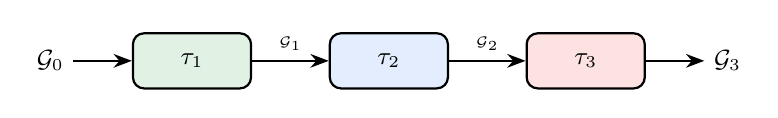
\begin{tikzpicture}[
  box/.style={draw, thick, rounded corners, minimum width=1.5cm, minimum height=0.7cm, font=\small},
  arr/.style={-{Stealth}, thick},
]
\node[box, fill=batch0!15] (a) at (0,0) {$\tau_1$};
\node[box, fill=batch1!15] (b) at (2.5,0) {$\tau_2$};
\node[box, fill=batch2!15] (c) at (5,0) {$\tau_3$};
\node[font=\small] (g0) at (-1.8,0) {$\mathcal{G}_0$};
\node[font=\small] (g3) at (6.8,0) {$\mathcal{G}_3$};
\draw[arr] (g0) -- (a);
\draw[arr] (a) -- node[above, font=\tiny] {$\mathcal{G}_1$} (b);
\draw[arr] (b) -- node[above, font=\tiny] {$\mathcal{G}_2$} (c);
\draw[arr] (c) -- (g3);
\end{tikzpicture}
\end{center}

\subsection{Parallel}

\begin{center}
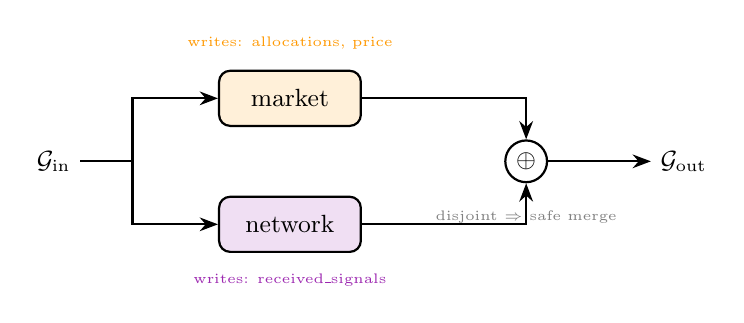
\begin{tikzpicture}[
  box/.style={draw, thick, rounded corners, minimum width=1.8cm, minimum height=0.7cm, font=\small},
  arr/.style={-{Stealth}, thick},
]
\node[font=\small] (gin) at (0,0) {$\mathcal{G}_\text{in}$};
\node[box, fill=market!15] (m) at (3, 0.8) {market};
\node[box, fill=network!15] (n) at (3,-0.8) {network};
\node[circle, draw, thick, inner sep=2pt, font=\small] (merge) at (6, 0) {$\oplus$};
\node[font=\small] (gout) at (8,0) {$\mathcal{G}_\text{out}$};

\draw[arr] (gin) -- ++(1,0) |- (m);
\draw[arr] (gin) -- ++(1,0) |- (n);
\draw[arr] (m) -| (merge);
\draw[arr] (n) -| (merge);
\draw[arr] (merge) -- (gout);

% Annotations
\node[font=\tiny, text=market, anchor=south] at (3, 1.3) {writes: allocations, price};
\node[font=\tiny, text=network, anchor=north] at (3, -1.3) {writes: received\_signals};
\node[font=\tiny, text=gray, anchor=north] at (6, -0.5) {disjoint $\Rightarrow$ safe merge};
\end{tikzpicture}
\end{center}

\subsection{Conditional}

\begin{center}
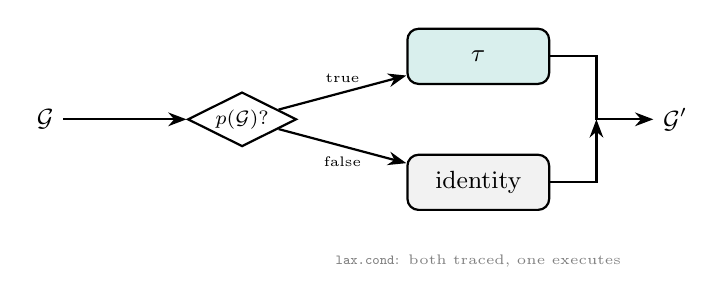
\begin{tikzpicture}[
  box/.style={draw, thick, rounded corners, minimum width=1.8cm, minimum height=0.7cm, font=\small},
  arr/.style={-{Stealth}, thick},
]
\node[font=\small] (gin) at (0,0) {$\mathcal{G}$};
\node[diamond, draw, thick, aspect=2, inner sep=1pt, font=\scriptsize] (pred) at (2.5,0) {$p(\mathcal{G})$?};
\node[box, fill=democracy!15] (yes) at (5.5, 0.8) {$\tau$};
\node[box, fill=gray!10] (no) at (5.5, -0.8) {identity};
\node[font=\small] (gout) at (8,0) {$\mathcal{G}'$};

\draw[arr] (gin) -- (pred);
\draw[arr] (pred) -- node[above, font=\tiny] {true} (yes);
\draw[arr] (pred) -- node[below, font=\tiny] {false} (no);
\draw[arr] (yes) -| (7, 0) -- (gout);
\draw[arr] (no) -| (7, 0);

\node[font=\tiny, text=gray, anchor=north] at (5.5, -1.6) {\texttt{lax.cond}: both traced, one executes};
\end{tikzpicture}
\end{center}

%% ================================================================
\section{Type Contracts}

Each mechanism type declares which \textsc{GraphState} fields it reads and writes.
Disjoint write sets enable safe parallel composition.

\begin{center}
\begin{tabular}{@{}llll@{}}
\toprule
\textbf{Type} & \textbf{Reads} & \textbf{Writes} & \textbf{Topology} \\
\midrule
Market & budget, market\_wts, resource & allocations, budget, price & Global hub \\
Network & signal, adj[network] & received\_signals & Local sparse \\
Democracy & vote\_wts, last\_harvest & harvest\_target, penalty\_$\lambda$ & All$\to$one$\to$all \\
\bottomrule
\end{tabular}
\end{center}

\noindent\textbf{Write disjointness:} Market writes $\{$allocations, budget, price$\}$.
Network writes $\{$received\_signals$\}$. Democracy writes $\{$target, $\lambda\}$.
Intersection = $\emptyset$ $\Rightarrow$ \texttt{parallel(market, network, democracy)} is valid.

%% ================================================================
\section{Fishing Commons State}

\begin{center}
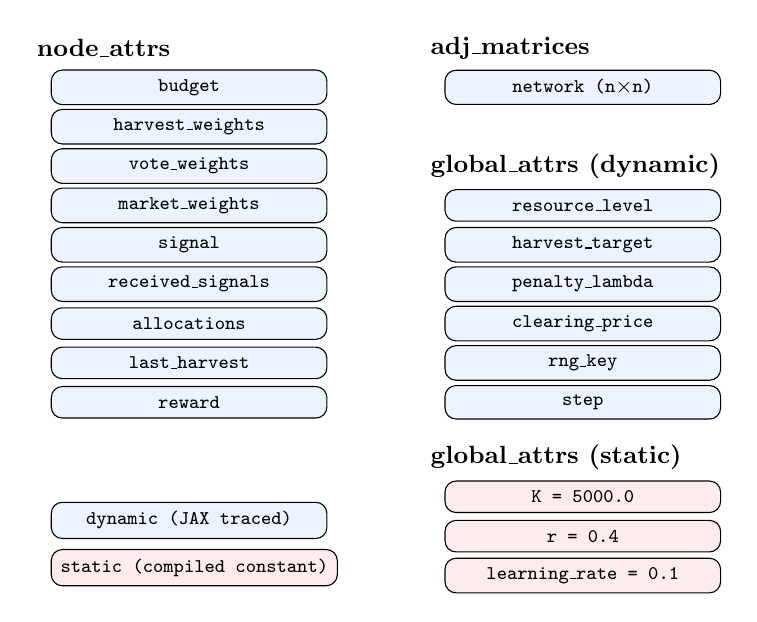
\begin{tikzpicture}[
  field/.style={draw, rounded corners, minimum width=3.5cm, minimum height=0.4cm,
                font=\scriptsize\ttfamily, anchor=west},
  label/.style={font=\small\bfseries, anchor=west},
]
% node_attrs
\node[label] at (0, 3.5) {node\_attrs};
\foreach \i/\name in {0/budget, 1/harvest\_weights, 2/vote\_weights,
                      3/market\_weights, 4/signal, 5/received\_signals,
                      6/allocations, 7/last\_harvest, 8/reward} {
  \node[field, fill=dynamic!10] at (0.3, 3.0-\i*0.5) {\name};
}

% adj_matrices
\node[label] at (5, 3.5) {adj\_matrices};
\node[field, fill=dynamic!10] at (5.3, 3.0) {network (n$\times$n)};

% global_attrs (dynamic)
\node[label] at (5, 2.0) {global\_attrs (dynamic)};
\foreach \i/\name in {0/resource\_level, 1/harvest\_target,
                      2/penalty\_lambda, 3/clearing\_price,
                      4/rng\_key, 5/step} {
  \node[field, fill=dynamic!10] at (5.3, 1.5-\i*0.5) {\name};
}

% global_attrs (static)
\node[label] at (5, -1.7) {global\_attrs (static)};
\foreach \i/\name in {0/K = 5000.0, 1/r = 0.4, 2/learning\_rate = 0.1} {
  \node[field, fill=static!10] at (5.3, -2.2-\i*0.5) {\name};
}

% Legend
\node[field, fill=dynamic!10] at (0.3, -2.5) {dynamic (JAX traced)};
\node[field, fill=static!10] at (0.3, -3.1) {static (compiled constant)};
\end{tikzpicture}
\end{center}

%% ================================================================
\section{Summary of Changes}

\begin{center}
\begin{tabular}{@{}lll@{}}
\toprule
\textbf{File} & \textbf{Change} & \textbf{Status} \\
\midrule
\texttt{core/graph.py} & Pytree fix: partition global\_attrs & Done \\
\texttt{core/category.py} & \texttt{@transform}, \texttt{parallel}, \texttt{conditional} & Done \\
\texttt{core/category.py} & Bug fixes: identity, sequential, compose metadata & Done \\
\texttt{core/pipeline.py} & Pipeline compiler (typed DAG) & Done \\
\texttt{core/schedule.py} & Schedule primitive (cadence + phase) & Done \\
\texttt{fishing\_commons/state.py} & Initial state factory & Done \\
\texttt{mechanisms/\_\_init\_\_.py} & Type contracts & Done \\
\bottomrule
\end{tabular}
\end{center}

\noindent\textbf{Remaining:} \texttt{lax.scan} episode runner, \texttt{vmap} over seeds,
mechanism implementations (market, network, democracy), resource dynamics,
reward, learning transforms, and the full 13,200-episode sweep.

\end{document}
